\documentclass[crop=true]{standalone}
\usepackage{pgfplots}
\usepgfplotslibrary{fillbetween}
\pgfplotsset{compat=1.15}
\usepackage{multido}

\begin{document}
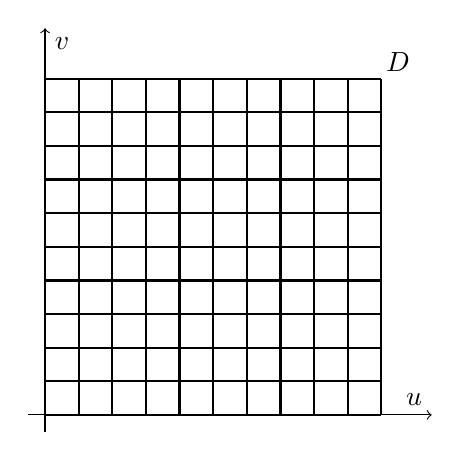
\begin{tikzpicture}[baseline=(ylabel.center)]
\begin{axis}[
axis on top,
axis lines = middle,
unit vector ratio*=1 1 1,
scale=0.9, xmin=-0.05, xmax=1.15, ymin=-0.05, ymax=1.15,
%grid = major,
xtick={0},
ytick={0},
%xticklabels = {1,2},
%yticklabels = {1,2},
xlabel=$u$,
ylabel=$v$,
ylabel style={name=ylabel},
axis line style = {->},
]
\multido{\i=0+1}{11}{
\addplot[samples=2,samples y=0,domain=0:1, thick]({x},{\i/10});
\addplot[samples=2,samples y=0,domain=0:1, thick]({\i/10},{x});
}
% \addplot[name path=up,samples=2,samples y=0,domain=0.3:0.4]({x},{0.2});
% \addplot[name path=down,samples=2,samples y=0,domain=0.3:0.4]({x},{0.1});
% \addplot[gray!50]fill between[of=up and down];
% \node at (axis cs:0.35,0.15){\small$\widehat{D}_{ij}$};
\node at (axis cs:1.05,1.05){$D$};
\end{axis}
\end{tikzpicture}

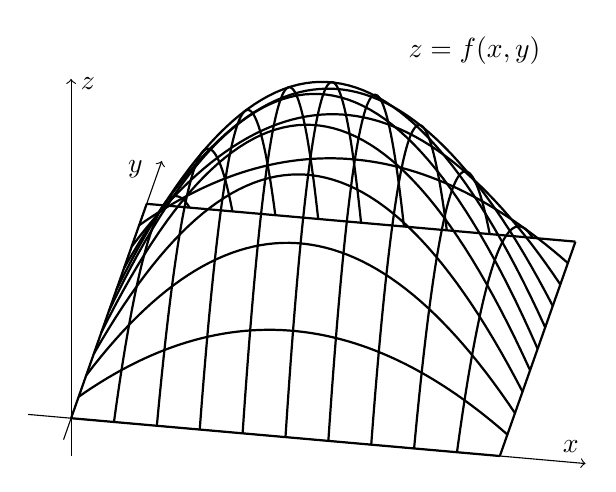
\begin{tikzpicture}[baseline=(zlabel.center)]
\begin{axis}[
axis on top,
axis lines = middle,
unit vector ratio*=1 1 1,
scale=2.1, xmin=-0.1, xmax=1.2, ymin=-0.1, ymax=1.2, zmin = -0.1, zmax = 0.9,
view={10}{30},
%grid = major,
xtick={0},
ytick={0},
ztick = {0},
xlabel=$x$,
ylabel=$y$,
zlabel = $z$,
zlabel style={name=zlabel},
axis line style = {->},
]
\multido{\i=0+1}{11}{
\addplot3[samples=60,samples y=0,domain=0:1, thick]({x},{\i/10},{(x*(x-1)*(\i/10)*(\i/10-1))*10});
\addplot3[samples=60,samples y=0,domain=0:1, thick]({\i/10},{x},{(x*(x-1)*(\i/10)*(\i/10-1))*10});
}
% \addplot3[name path=up,samples=10,samples y=0,domain=0.3:0.4]({x},{0.2},{x*(1-x)*0.16*10});
% \addplot3[name path=down,samples=10,samples y=0,domain=0.3:0.4]({x},{0.1},{x*(1-x)*0.09*10});
% \addplot[gray!50]fill between[of=up and down];
% \node at (axis cs:0.35,0.15,0.25){$D_{ij}$};
\node at (axis cs:0.8,0.8,0.6){$z = f(x, y)$};
\end{axis}
\end{tikzpicture}

\end{document}